\documentclass{article}

\usepackage[final]{style}
\usepackage[utf8]{inputenc} % allow utf-8 input
\usepackage[T1]{fontenc}    % use 8-bit T1 fonts
\usepackage{hyperref}       % hyperlinks
\usepackage{url}            % simple URL typesetting
\usepackage{booktabs}       % professional-quality tables
\usepackage{amsfonts}       % blackboard math symbols
\usepackage{nicefrac}       % compact symbols for 1/2, etc.
\usepackage{microtype}      % microtypography
\usepackage{verbatim}
\usepackage{graphicx}       % for figures
\usepackage{subcaption}

\title{Lecture 15: Detecting Objects by Parts}

\author{
  David R. Morales, Austin O. Narcomey, Minh-An Quinn, Guilherme F. Reis, Omar Solis \\
  Department of Computer Science\\
  Stanford University\\
  Stanford, CA 94305 \\
  \texttt{\{dmorales, \}@cs.stanford.edu} \\
}

\begin{document}

\maketitle


\section{Introduction to Object Detection}

\section{Current Object Detection Benchmarks}

\section{Evaluating Object Detection}

\section{A Simple Sliding Window Detector}
An approach to the detection problem is to treat it as a classification problem. Instead of attempting to produce the location of objects in an image by processing the entire image at once, slide a window over the image and classify each position of the window as either containing an object or not (figure X).

\begin{figure}[h]
  \begin{subfigure}{0.48\textwidth}
    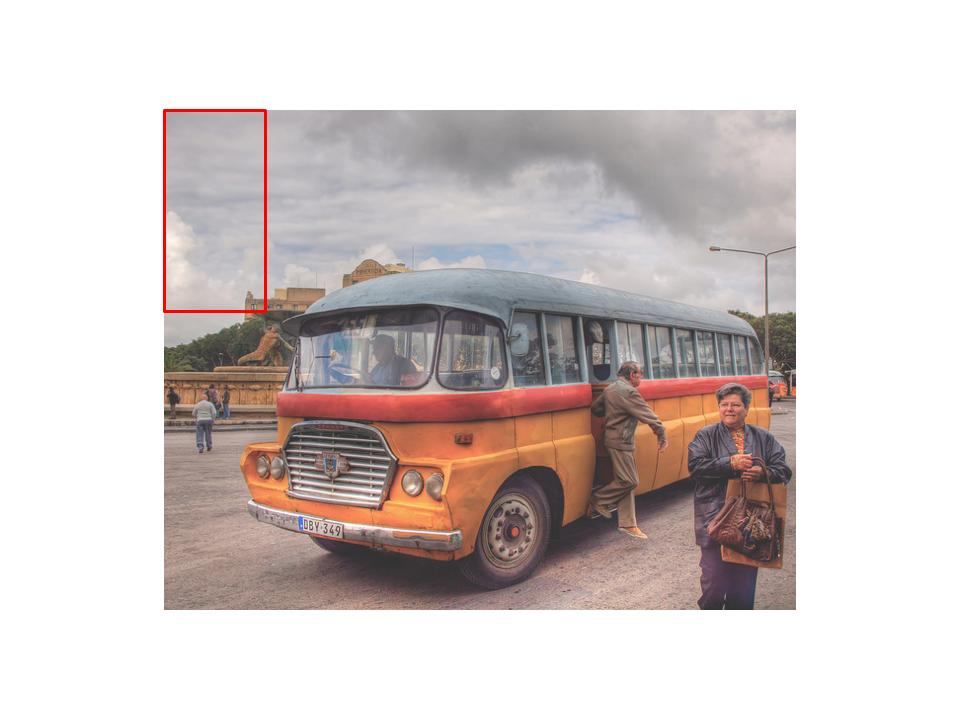
\includegraphics[width=\linewidth]{sliding_window_a.jpg}
    \caption{}
  \end{subfigure}
  \hspace*{\fill} % separation between the subfigures
  \begin{subfigure}{0.48\textwidth}
    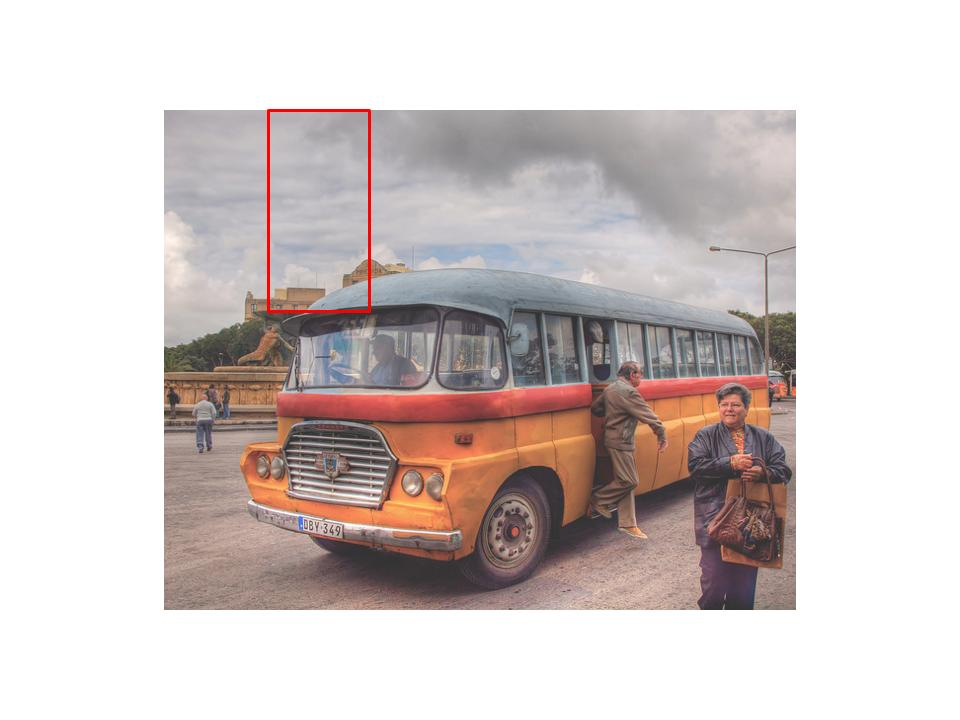
\includegraphics[width=\linewidth]{sliding_window_b.jpg}
    \caption{}
  \end{subfigure}
  \hspace*{\fill} % separation between the subfigures
  \begin{subfigure}{0.48\textwidth}
    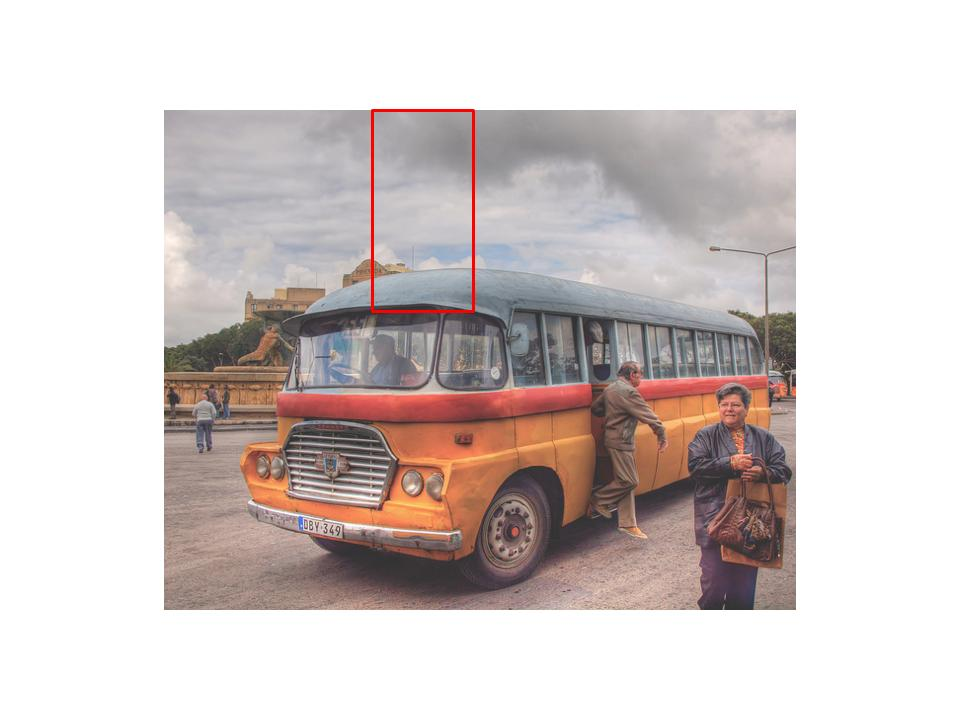
\includegraphics[width=\linewidth]{sliding_window_c.jpg}
    \caption{}
  \end{subfigure}
  \hspace*{\fill} % separation between the subfigures
  \begin{subfigure}{0.48\textwidth}
    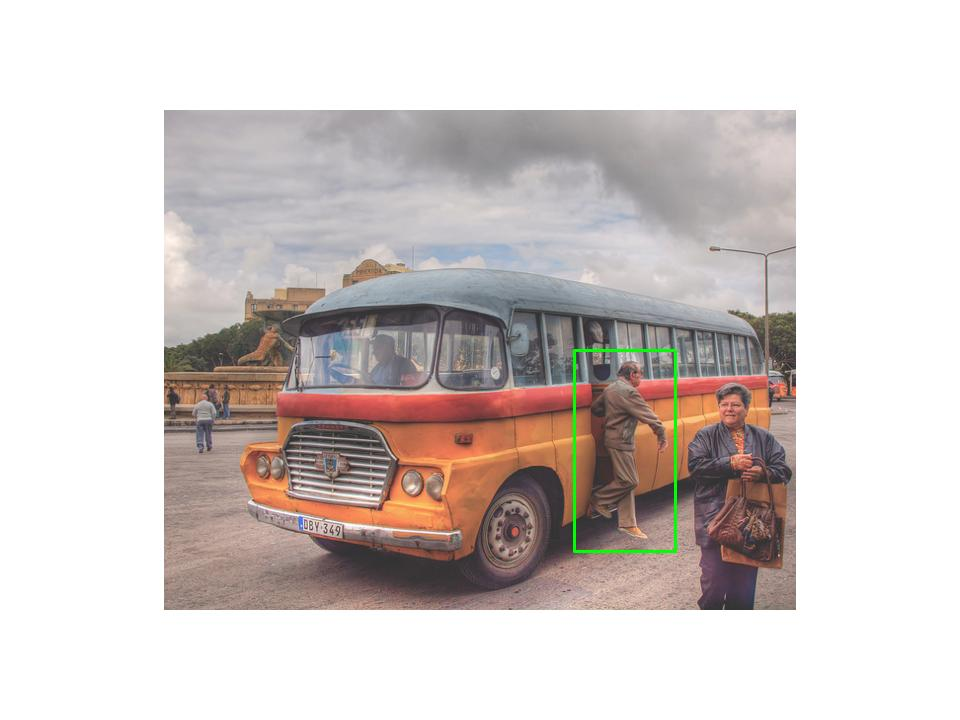
\includegraphics[width=\linewidth]{sliding_window_d.jpg}
    \caption{}
  \end{subfigure}
  \caption{Consider the problem of detecting people in an image. (a) - (c) Sliding window across image and at each position classifying window as not containing a person. (b) Window over person and classifying window as containing a person. Image source: Flickr user neilalderney123}
\end{figure}

\subsection{Feature Extraction and Object Representation}
Dalal and Triggs \cite{hog_human_detection} show the effectiveness of using Histograms of Oriented Gradient (HOG) descriptors for human detection. Although their feature extraction methods were focused on human detection, they can be applied for detecting various objects. 

Recall HOG descriptors from lecture 8. Essentially, an image window is divided into blocks and the magnitude of the gradients of the pixels in each block are accumulated into bins according to the direction of the gradients. These local histograms of the blocks are then normalized and concatenated to produce a feature representation of the the image window.

\begin{figure}[h]
	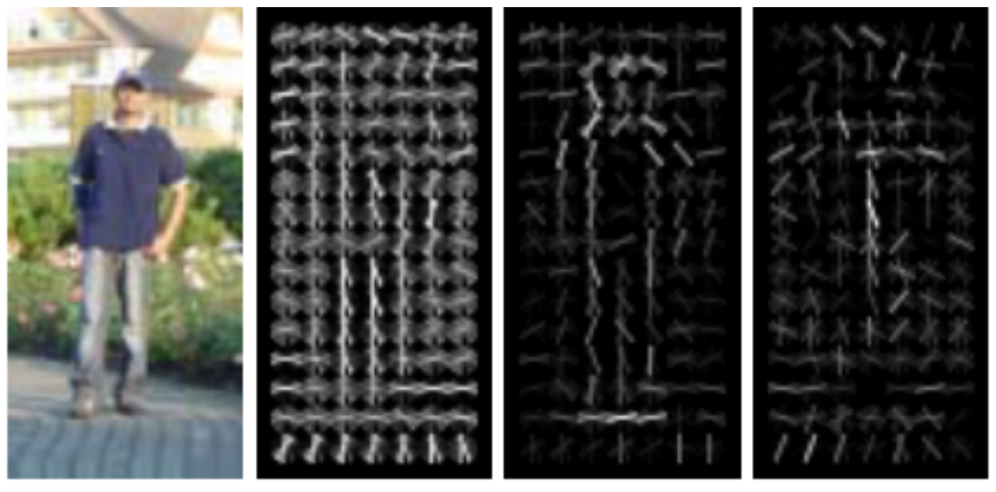
\includegraphics[width=\linewidth, scale=0.3]{person_template.png}
	\caption{An image of a person along with its respective HOG descriptor. Note that the last two images the HOG descriptor weighted by the positive and negative weights of the classifier using them. The outline of the person is very visible in the weighted descriptors. Image source: Dalal and Triggs \cite{hog_human_detection}}
\end{figure}

Figure X shows an example of transforming an image into a HOG feature space. Producing a prototypical representation of an object would then involve considering many image windows labeled with containing that object. One approach to creating this representation would be to train a classifier on the HOG descriptors of these many labeled image windows and then proceed to use the trained classifier too classify the windows in images of interest. In their aim to improve human detection, for example, Dalal and Triggs \cite{hog_human_detection} train a linear Support Vector Machine on the HOG descriptors of image windows containing people.

A more simple approach, and the approach that will be assumed below, is that of averaging the window images containing an object of interest and then extracting the HOG descriptor of that average image to create a template for the object (Figure X).

\begin{figure}[h]
	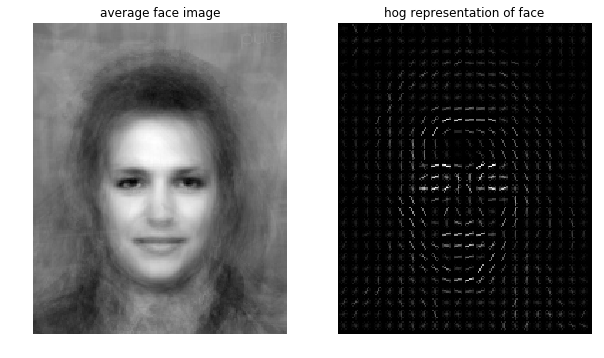
\includegraphics[width=\linewidth]{average_face_template.png}
	\caption{The average face image above is created by averaging 31 aligned face images of the same size. The HOG descriptor of this average face image can then be used as a template for detecting faces in images.}
\end{figure}


\subsection{Classifying Windows}
Now that we have a method for extracting useful features from an image window and for constructing object templates, we can proceed to detecting objects in images. The idea is to compare each window with the object template and search for matches. That is, the object template itself acts as a filter that slides across the image. At each position, the HOG descriptor of the window being compared is extracted and a similarity score between the two HOG descriptors is computed. If the similarity score at some location is above a predefined detection threshold, then an object can be said to have been detected in the window at that location.

DISCUSS HOW SIMILARY IS SCORED?

As effective as the method seems so far, it's success is very limited by the size of the sliding template window. For example, consider when there are objects that are larger than the template being used to detect them (Figure X).

\begin{figure}[h]
  \begin{subfigure}{0.48\textwidth}
    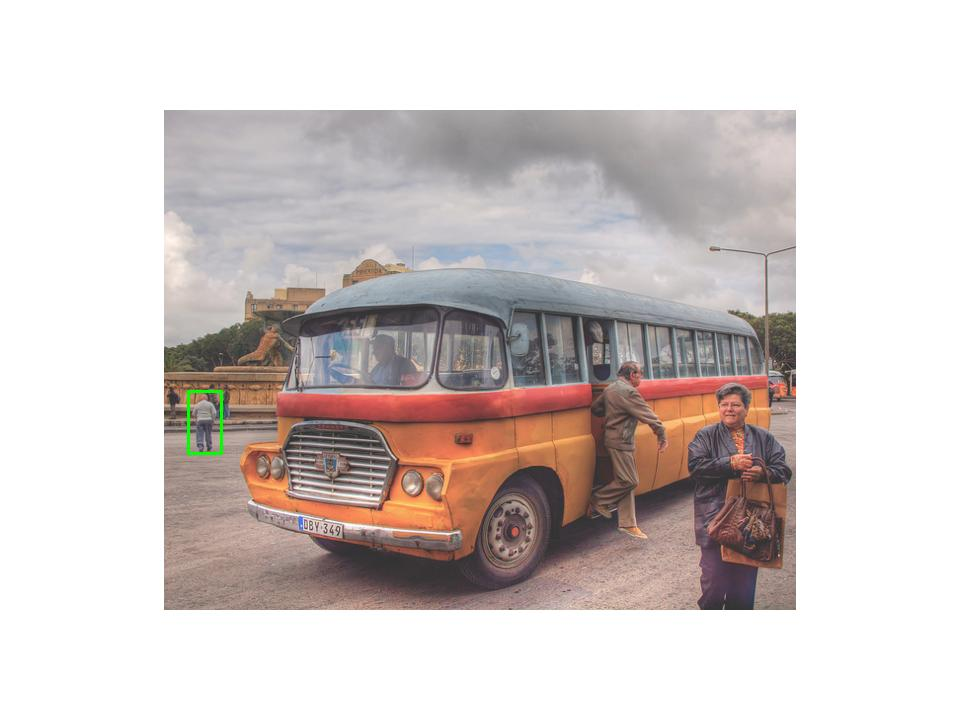
\includegraphics[width=\linewidth]{small_sliding_window_a.jpg}
    \caption{}
  \end{subfigure}
  \hspace*{\fill} % separation between the subfigures
  \begin{subfigure}{0.48\textwidth}
    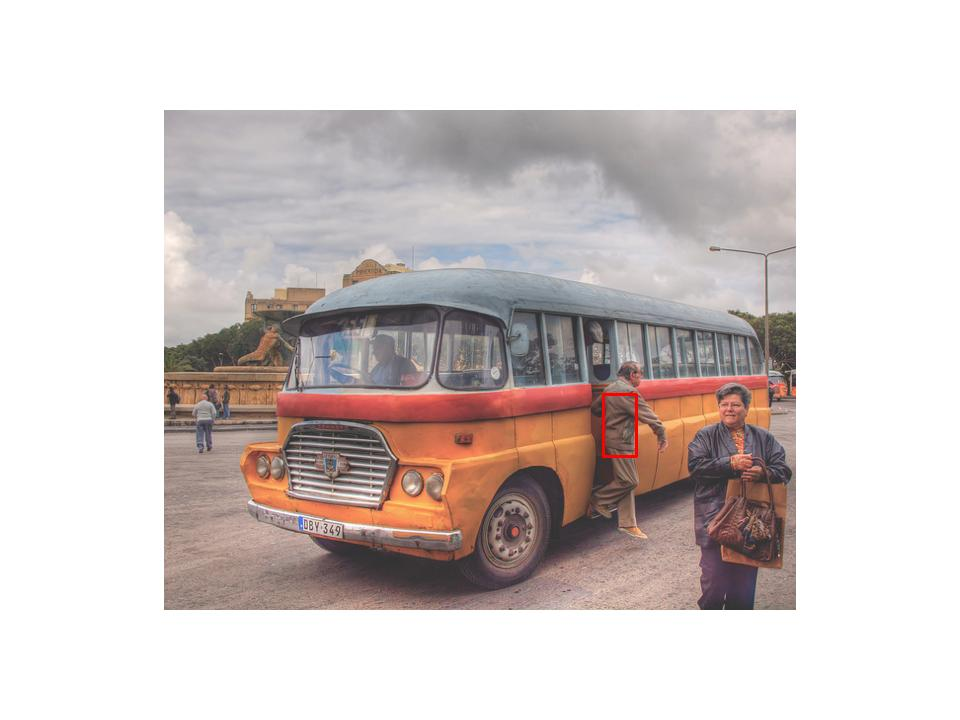
\includegraphics[width=\linewidth]{small_sliding_window_b.jpg}
    \caption{}
  \end{subfigure}
  \caption{Consider, again the problem of detecting people, except this time our sliding window is much smaller. (a) The template and sliding window are still large enough to detect the smaller, distant person. (b) The person in the foreground is a lot bigger than our window size and is not being detected.}
\end{figure}

\subsection{Multi Scale Sliding Window}
To account for variations in size of the objects being detected, multiple scalings of the the image are considered. Essentially, a feature pyramid (Figure X) of different image resizings is created. The sliding window technique is then applied as usual over all the levels of the pyramid. The window that produces the highest similarity score out of the resizings is used as the location of the detected object.

\begin{figure}[h]
	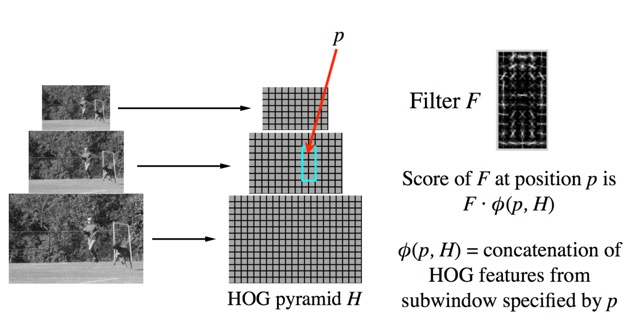
\includegraphics[width=\linewidth]{feature_pyramid.jpg}
	\caption{Using a feature pyramid of different image resizings allows the object template to match with objects that might originally have been bigger to much smaller than the the template. Image source: Lecture 15, Slide 40}.
\end{figure}

\subsection{Issues}
- Method is too strict in terms of how objects must appear in image (orientation and shape...)


\section{The Deformable Parts Model (DPM)}

\section{The DPM Detection Pipeline}

\section{DPM Detection Results}



% References
\small
\bibliographystyle{plain}
\bibliography{bibliography}
\cite{hog_human_detection}
\end{document}
